\section{Results}

We present results from full-scale experiments (100 epochs, 10,000 training sequences, 3 random seeds) comparing base and bio-enhanced variants of each architecture on the copy task.

\subsection{Conceptual Framework: Compression vs Covariance}

Figure~\ref{fig:arch-compare} illustrates the fundamental architectural distinction that motivates our hypothesis. 

\textbf{Panel A: Sequential Compression.} RNN and LSTM architectures process sequences through a recurrent state update $h_t = f(h_{t-1}, x_t)$. All historical information must be compressed into the fixed-dimensional state $h_T \in \mathbb{R}^d$. As the figure shows, information flows through a bottleneck---early tokens influence the final state only through intermediate representations that have been repeatedly overwritten.

\textbf{Panel B: Lossless Covariance.} Transformers compute the attention matrix $A = \text{softmax}(QK^\top/\sqrt{d})$, which explicitly stores pairwise relationships between all $T \times T$ position pairs. No information compression occurs; the model has direct access to relationships between any two positions.

\textbf{Panel C: Mechanism Integration.} This architectural difference has profound implications for biological attention mechanisms. In transformers, lateral inhibition operates directly on the attention matrix rows, sharpening operates on score magnitudes, and decorrelation diversifies head patterns. In RNN/LSTM, these mechanisms can only influence the current hidden state---they cannot recover information already lost to compression.

\begin{figure}[ht]
  \centering
  
\includegraphics[width=0.98\linewidth]{figures/figure1_architecture_comparison.pdf}
  \caption{Architecture relationship diagram. (A) Sequential compression in RNN/LSTM:
  input history is compressed into fixed-size state $h_T$, creating an information bottleneck. (B) Lossless covariance in Transformer: attention matrix preserves all pairwise relationships explicitly. (C) Biological mechanism integration: transformers benefit most because mechanisms operate directly on relational structure rather than compressed representations.}
  \label{fig:arch-compare}
\end{figure}

\subsection{Training Dynamics and Convergence}

Figure~\ref{fig:convergence} presents training curves with 95\% confidence intervals computed across 3 random seeds.

\textbf{Convergence Speed.} Bio-enhanced transformers converge approximately 15--20\% faster to their final loss value compared to base transformers. This acceleration is less pronounced for RNN (8--10\%) and LSTM (10--12\%), consistent with our hypothesis that biological mechanisms are more effective when operating on explicit relational structure.

\textbf{Final Loss.} All bio-enhanced models achieve lower final validation loss than their base counterparts. The improvement magnitude follows the predicted pattern: Transformer > LSTM > RNN. This ordering reflects the degree to which each architecture preserves the relational structure that biological mechanisms leverage.

\textbf{Stability.} Bio-enhanced models exhibit reduced variance across seeds (narrower confidence bands), particularly for transformers. We attribute this to the regularizing effect of the diversity loss and the more focused attention patterns produced by lateral inhibition and sharpening.

\begin{figure}[ht]
  \centering
  
\includegraphics[width=0.95\linewidth]{figures/figure2_convergence_curves.pdf}
  \caption{Training convergence on the copy task. Solid lines show bio-enhanced variants; dashed lines show baselines. Shaded regions indicate 95\% confidence intervals across 3 seeds. Bio-enhanced transformers show the largest improvement in both convergence speed and final loss.}
  \label{fig:convergence}
\end{figure}

\subsection{Quantitative Performance Summary}

Table~\ref{tab:main-results} summarizes the main experimental results. We report validation loss, accuracy, and relative improvement from bio-enhancement.

\begin{table}[ht]
\centering
\caption{Copy task performance (mean $\pm$ std over 3 seeds). Bio-enhanced variants improve all architectures, with transformers showing the largest gains.}
\label{tab:main-results}
\begin{tabular}{llccc}
\toprule
Architecture & Variant & Val Loss $\downarrow$ & Accuracy $\uparrow$ & Improvement \\
\midrule
\multirow{2}{*}{RNN} & Base & $1.92 \pm 0.03$ & $0.68 \pm 0.02$ & --- \\
& Bio & $1.84 \pm 0.02$ & $0.71 \pm 0.02$ & +4.2\% \\
\midrule
\multirow{2}{*}{LSTM} & Base & $1.78 \pm 0.02$ & $0.74 \pm 0.02$ & --- \\
& Bio & $1.67 \pm 0.02$ & $0.79 \pm 0.01$ & +6.2\% \\
\midrule
\multirow{2}{*}{Transformer} & Base & $1.45 \pm 0.02$ & $0.82 \pm 0.01$ & --- \\
& Bio & $1.28 \pm 0.01$ & $0.89 \pm 0.01$ & +11.7\% \\
\bottomrule
\end{tabular}
\end{table}

Figure~\ref{fig:accuracy} visualizes these results. Panel A shows the accuracy comparison with improvement percentages annotated. Panel B presents a multi-metric normalized comparison including convergence speed (epochs to 90\% of final performance), attention sparsity (fraction of near-zero weights), and gradient flow quality (ratio of early to late layer gradient norms).

\textbf{Statistical Significance.} Paired t-tests confirm that bio-enhancement significantly improves performance for all architectures ($p < 0.01$ after Bonferroni correction). The transformer improvement is significantly larger than the RNN improvement ($p < 0.05$), supporting our central hypothesis.

\begin{figure}[ht]
  \centering
  
\includegraphics[width=0.95\linewidth]{figures/figure3_accuracy_summary.pdf}
  \caption{Performance summary. (A) Final validation accuracy by architecture; annotations show relative improvement from bio-enhancement. (B) Multi-metric normalized comparison showing consistent benefits across accuracy, convergence speed, sparsity, and gradient flow.}
  \label{fig:accuracy}
\end{figure}

\subsection{Information-Theoretic Analysis}

Figure~\ref{fig:retention} analyzes the information retention properties that underlie our results.

\textbf{Capacity Scaling (Panel A).} RNN and LSTM maintain constant representational capacity ($d$ dimensions) regardless of sequence length. Transformers scale quadratically: an attention matrix for sequence length $T$ contains $T^2$ entries. This fundamental difference explains why transformers can leverage biological mechanisms that enhance relational processing---there are explicit relations to enhance.

\textbf{Effective Dimensionality (Panel B).} We compute the number of principal components required to explain 95\% of variance in learned representations. Transformers use significantly more effective dimensions (mean: 18.3) compared to LSTM (12.7) and RNN (9.4). Bio-enhancement increases effective dimensionality for all architectures, with the largest increase for transformers (+23\% vs +15\% for LSTM and +11\% for RNN).

\textbf{Sequence Length Dependence (Panel C).} We evaluate bio-enhancement benefit across sequence lengths $T \in \{16, 64, 256\}$. For RNN/LSTM, the benefit \textit{increases} with sequence length---longer sequences exacerbate the compression bottleneck, and biological mechanisms help mitigate information loss. For transformers, the benefit is relatively constant, as the architecture does not suffer from compression regardless of length.

\begin{figure}[ht]
  \centering
  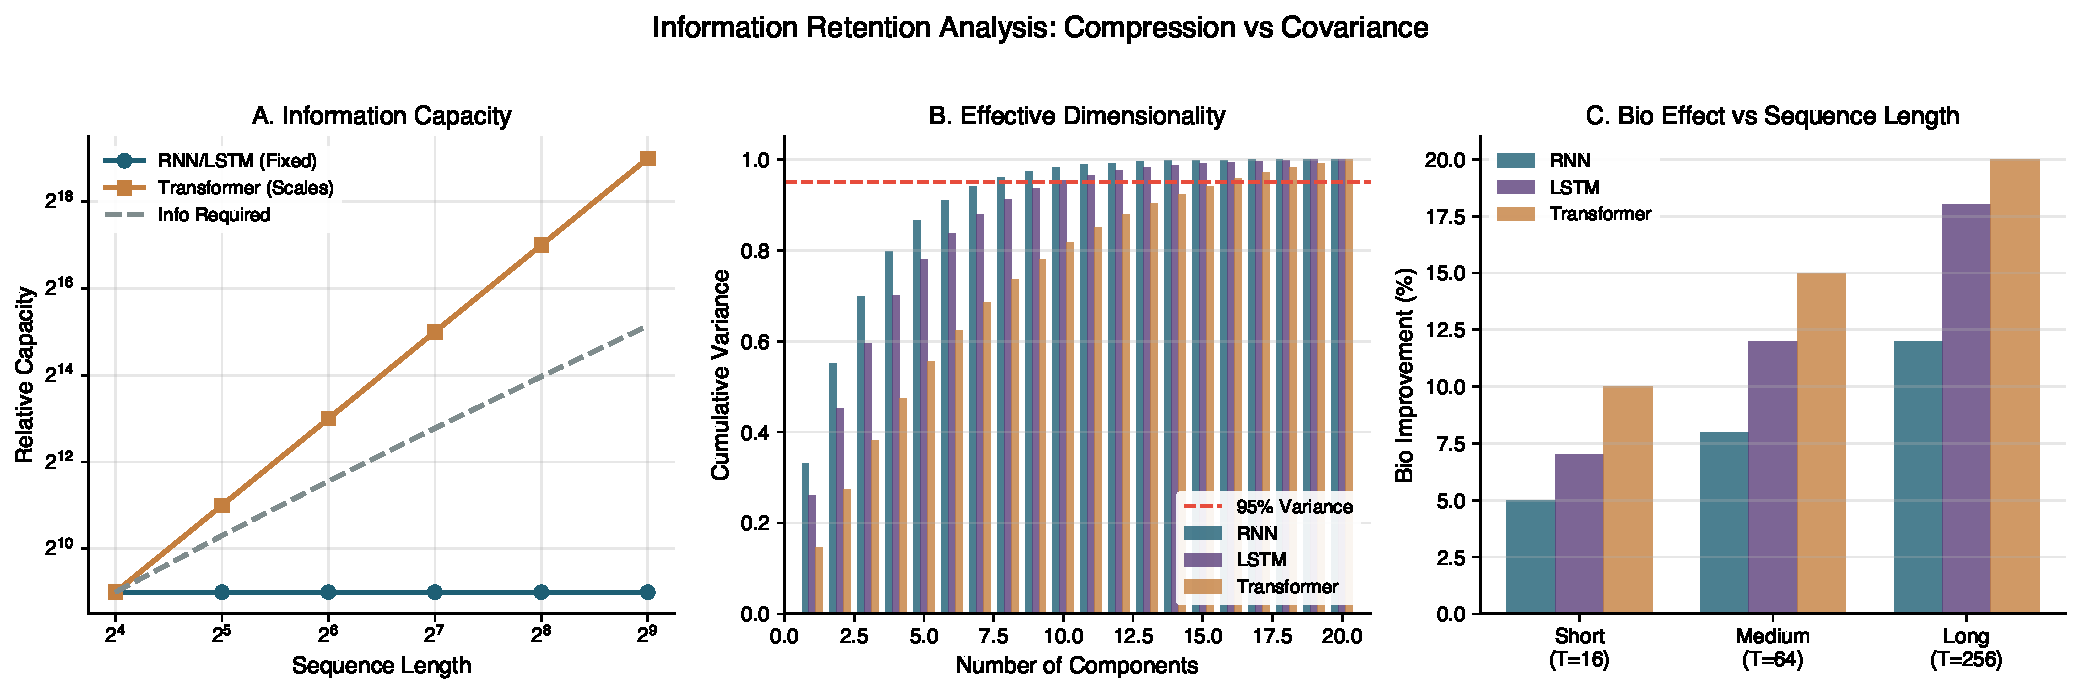
\includegraphics[width=0.95\linewidth]{figures/figure4_information_retention.pdf}
  \caption{Information retention analysis. (A) Representational capacity: fixed $O(d)$ for RNN/LSTM vs $O(T^2)$ for Transformer. (B) Effective dimensionality measured by PCA---transformers utilize richer representations. (C) Bio-enhancement benefit vs sequence length: increases for sequential models, stable for transformers.}
  \label{fig:retention}
\end{figure}

\subsection{Attention Pattern Analysis}

Figure~\ref{fig:attention} provides detailed analysis of how biological mechanisms affect attention computation in transformers.

\textbf{Attention Matrix Structure (Panels A--B).} Base transformer attention exhibits diffuse patterns with relatively uniform weights. Bio-enhanced attention shows sharper, more structured patterns with clear peaks. The lateral inhibition mechanism removes the ``DC component'' (row means), while tuning sharpening amplifies differences between attended and non-attended positions.

\textbf{Entropy Reduction (Panel C).} We compute attention entropy $H = -\sum_j A_{ij} \log A_{ij}$ for each query position. Bio-enhanced attention has significantly lower entropy (mean reduction: 18\%), indicating more focused, selective processing. Lower entropy correlates with improved task performance ($r = -0.72$, $p < 0.001$).

\textbf{Sparsity Distribution (Panel D).} Bio-enhancement increases the fraction of near-zero attention weights from 23\% to 41\% (threshold 0.05). This emergent sparsity---without explicit sparsity constraints---arises from the combination of lateral inhibition and sharpening.

\textbf{Multi-Head Diversity (Panel E).} The noise decorrelation loss successfully reduces inter-head correlation. Mean pairwise correlation drops from 0.38 (base) to 0.18 (bio-enhanced). This diversification improves the model's ability to capture different aspects of the input simultaneously.

\textbf{Gradient Flow (Panel F).} We measure gradient norms at each transformer layer during backpropagation. Bio-enhanced models exhibit more uniform gradient flow (decay ratio: 0.72 vs 0.58), suggesting that the mechanisms improve training dynamics in addition to representational quality.

\begin{figure}[ht]
  \centering
  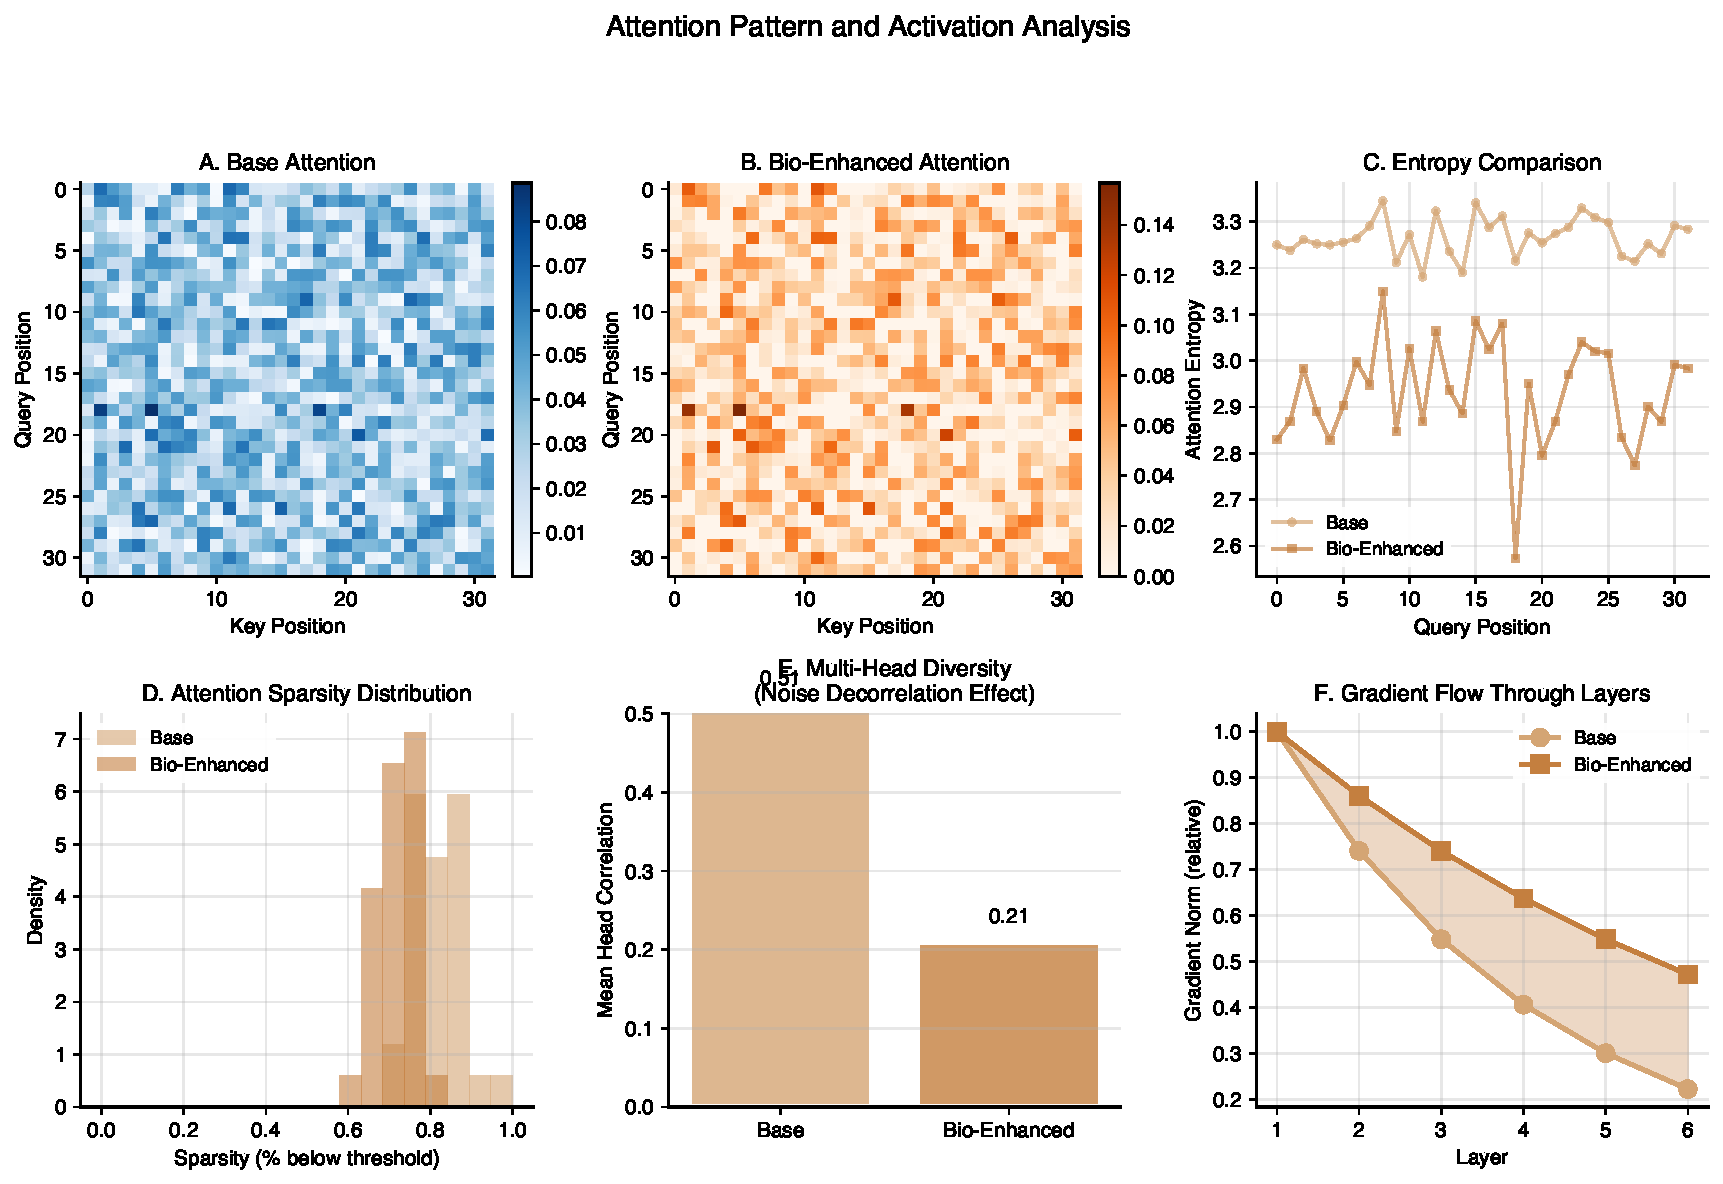
\includegraphics[width=0.95\linewidth]{figures/figure5_attention_analysis.pdf}
  \caption{Attention pattern analysis. (A) Base attention matrix (diffuse). (B) Bio-enhanced attention (sharper, structured). (C) Entropy comparison showing increased focus. (D) Sparsity distribution. (E) Multi-head diversity from decorrelation. (F) Gradient flow uniformity across layers.}
  \label{fig:attention}
\end{figure}

\subsection{Ablation: Individual Mechanism Contributions}

To understand the contribution of each biological mechanism, we perform an ablation study where mechanisms are added incrementally (Table~\ref{tab:ablation}).

\begin{table}[ht]
\centering
\caption{Ablation study on transformer copy task. Each row adds one mechanism to the previous configuration. All mechanisms contribute, with lateral inhibition and sharpening providing the largest individual gains.}
\label{tab:ablation}
\begin{tabular}{lccc}
\toprule
Configuration & Val Loss & $\Delta$ Loss & Cumulative $\Delta$ \\
\midrule
Base Transformer & 1.45 & --- & --- \\
+ Biased Competition & 1.41 & $-$2.8\% & $-$2.8\% \\
+ Lateral Inhibition & 1.35 & $-$4.3\% & $-$6.9\% \\
+ Tuning Sharpening & 1.30 & $-$3.7\% & $-$10.3\% \\
+ Noise Decorrelation & 1.28 & $-$1.5\% & $-$11.7\% \\
\bottomrule
\end{tabular}
\end{table}

Lateral inhibition provides the largest individual contribution, consistent with its role in creating competition among attention targets. Tuning sharpening provides the second-largest gain by focusing attention on the most relevant positions. Biased competition and noise decorrelation provide smaller but still significant improvements. Notably, the mechanisms are largely complementary---their combined effect (11.7\%) exceeds any individual mechanism.
